% This example An LaTeX document showing how to use the l3proj class to
% write your report. Use pdflatex and bibtex to process the file, creating 
% a PDF file as output (there is no need to use dvips when using pdflatex).

% Modified 

\documentclass{l3proj}
\begin{document}
\title{Team V - How Not To Kill Your Dog}
\author{Ross Adam \\
        Andrew Gardner \\
        Nicole Kearns \\
        Mamas Nicolaou \\
        Asset Sarsengaliyev}
\date{18 March 2013}
\maketitle

\chapter{Requirements}
\label{req}

\section{Client Interview}

The project was proposed by Dr Fiona Dowell, a senior lecturer at the University of Glasgow School of Veterinary Medicine. Initially, we met with Dr Fiona Dowell in order to gain more information about the requirements and specification for the application to ensure that we produced an application relevant to what the client wanted.\\
Our initial requirements for the vet application were :

\begin{itemize}
\item A learning application for vet students, providing step-by-step tutorials for different sections of the vet course.
\item Simple example questions within each topic to test how much the user is learning about that specific section.
\item A larger assessment at the end of all sections to test users on all the content within the application.
\end{itemize}

After the initial meeting with our client, we thought that it would be useful for the content within the application to be able to be updated , for example if the content changed; to fix errors or update to include different questions. We presented this idea to the client who agreed that this would be a useful feature as it might be good to be able to update after some user feedback. The functional requirements were then updated to include an administration system.\\
The administration system allows admin staff to upload and remove topics. It also allows the content of each topic to be updated, slides and questions can be added and removed.


\section{Functional Requirements}

\subsection{Requirements Table}

\textbf{Student -} Uses the application to browse through the different topics, answering the sample questions as they go along and completing the assessment at the end of all topics.

\textbf{User Admin -} Responsible for adding new users to the system, setting their permissions to determine their access levels and deleting them when necessay.

\textbf{Content Admin -} Responsible for adding new topics, slides and questions to the system, and ensuring that all content is kept up to date with the course content.

\textbf{Student}\\

\begin{center}
\begin{tabular}{|c|c|}
\hline \textbf{Id} & \textbf{Requirement}\\
\hline SR1 & View Topic\\
\hline SR2 & View Slides\\
\hline SR3 & View Questions\\
\hline SR4 & Answer Questions\\
\hline 
\end{tabular}
\end{center}

\textbf{User Admin}\\

\begin{center}
\begin{tabular}{|c|c|}
\hline \textbf{Id} & \textbf{Requirement}\\
\hline UAR1 & Add User\\
\hline UAR2 & Delete User\\
\hline UAR3 & Set Permissions\\
\hline 
\end{tabular}
\end{center}

\textbf{Content Admin}\\

\begin{center}
\begin{tabular}{|c|c|}
\hline \textbf{Id} & \textbf{Requirement}\\
\hline CAR1 & Add Topic\\
\hline CAR2 & Edit Topic\\
\hline CAR3 & Delete Topic\\
\hline CAR4 & Add Slide\\
\hline CAR5 & Delete Slide\\
\hline CAR6 & Add Questions\\
\hline CAR7 & Edit Questions\\
\hline CAR8 & Delete Questions\\
\hline 
\end{tabular}
\end{center}


\subsection{Use Case Diagrams}

\begin{center}
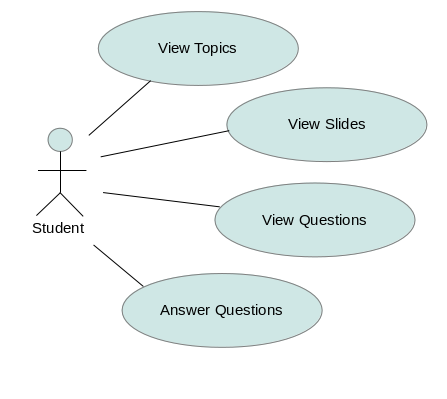
\includegraphics
[scale=0.5]
{/users/level3/0902059k/Level3/TP3/team-project/Dissertation/images/Student.png}
\end{center}
\begin{center} Student \end{center}

\begin{center}
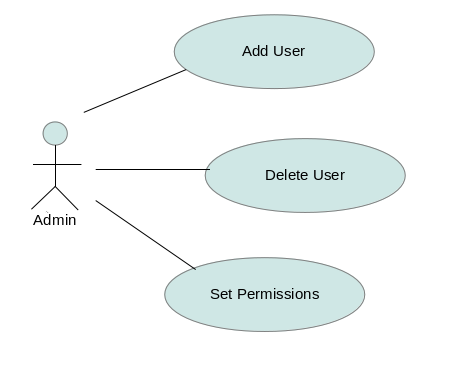
\includegraphics
[scale=0.5]
{/users/level3/0902059k/Level3/TP3/team-project/Dissertation/images/UserAdmin.png}
\end{center}
\begin{center} User Admin \end{center}

\begin{center}
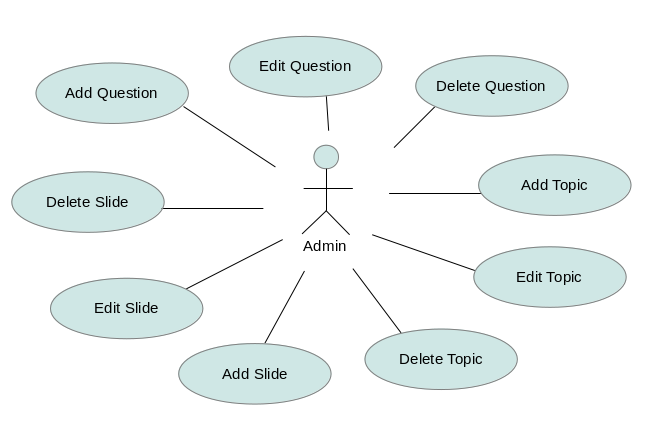
\includegraphics
[scale=0.5]
{/users/level3/0902059k/Level3/TP3/team-project/Dissertation/images/ContentAdmin.png}
\end{center}
\begin{center} Content Admin \end{center}

\subsection{Student Requirement Details}

\textbf{SR1: View Topics}\\
\textbf{Description}: Users must be able to view the different topics in the application. \\
\textbf{Rationale}: The students must be able to view the different topics in the application. This will allow them to navigate through the different topics as the progress through the slides and topics.\\
\textbf{Priority}: Must Have \\


\textbf{SR2: View Slides}\\
\textbf{Description}: Users must be able to view the different slides in the application. \\
\textbf{Rationale}: The students must be able to view the different slides in the learning application. The student will be able to navigate back and forward through the different slides of a topic and read through the content on each page.  \\
\textbf{Priority}: Must Have\\


\textbf{SR3: View Questions}\\
\textbf{Description}: Users must be able to view the different questions in the application. \\
\textbf{Rationale}: The student must be able to view the questions in the application. This will allow the students to go through the different questions related to the information given in the slides.\\
\textbf{Priority}: Must Have\\


\textbf{SR4: Answer Questions}\\
\textbf{Description}: Users must be able to answer the questions in the application.\\
\textbf{Rationale}: The student must be able to answer the questions in the learning application. This will allow the students to test the knowledge they learned from the information provided in the slides. \\
\textbf{Priority}: Must Have\\
\textbf{Dependencies}: SR3\\


\subsection{User Admin Requirements Details}

\textbf{UAR1: Add User} \\
\textbf{Description}: The admin user must be able to add a user.  \\
\textbf{Rationale}: The admin users must be able to create a new user account to allow other users to use the application and have access to the content management.\\
\textbf{Priority}: Must have \\

\textbf{UAR2: Delete User} \\
\textbf{Description}: The admin user should be able to delete a user. \\ 
\textbf{Rationale}: The admin user should be able to remove users from the system, meaning that they will no longer be able to login or have access to any of the content management.\\
\textbf{Priority}: Should have \\
\textbf{Dependencies}: UAR1\\

\textbf{UAR3: Set Permission} \\
\textbf{Description}: The admin user must be able to set user permissions.\\
\textbf{Rationale}: The admin user must be able to set user permissions in order to provide users with the appropriate access.\\
\textbf{Priority}: Must have \\
\textbf{Dependencies}: UAR1\\

\subsection{Content Admin Requirements Details}

\textbf{CAR1: Add Topic}\\
\textbf{Description}:  The admin users must be able to add a new topic. \\
\textbf{Rationale}: The admin user must be able to create a new topic within the admin site. \\
\textbf{Priority}: Must have\\


\textbf{CAR2: Edit Topic}\\
\textbf{Description}: The admin users should be able to edit a current topic.\\
\textbf{Rationale}: The admin user should be able to edit a current topic for the application. This will allow the admin user to update the topic if it any details change or are inaccurate.\\
\textbf{Priority}: Should Have \\
\textbf{Dependencies}: CAR1\\

\textbf{CAR3: Delete Topic}\\
\textbf{Description}: The admin users must be able to delete a current topic. \\
\textbf{Rationale}: The admin users must be able to remove a current topic from the application. This will mean that the topic will no longer be available within the application.\\
\textbf{Priority}: Must Have \\
\textbf{Dependencies}: CAR1\\

\textbf{CAR4: Add Slide}\\
\textbf{Description}:  The admin users must be able to add a new slide. \\
\textbf{Rationale}: The admin users must be able to add new slides to the application. This will provide the content for the students to browse through. \\
\textbf{Priority}: Must Have\\

\textbf{CA56: Delete Slide}\\
\textbf{Description}: The admin users must be able to delete a slide.\\ 
\textbf{Rationale}: The admin users must be able to remove a slide from the application. This means that selected slide will no longer be available in the application.\\
\textbf{Priority}: Must have\\
\textbf{Dependencies}: CAR4\\

\textbf{CAR6: Add Question}\\
\textbf{Description}: The admin users must be able to add questions to the application. \\
\textbf{Rationale}: The admin users must be able to create new questions and add them to the application, allowing the students to test how much they have learned.\\
\textbf{Priority}: Must Have\\

\textbf{CAR7: Edit Question}\\
\textbf{Description}: The admin users should be able to edit questions.\\
\textbf{Rationale}: The admin users should be able to edit questions. The users should be able to update the questions to keep the questions up to date or to fix error.\\
\textbf{Priority}: Should Have \\
\textbf{Dependencies}: CAR6\\

\textbf{CAR8: Delete Question}\\
\textbf{Description}: The admin user must be able to delete questions. \\
\textbf{Rationale}:  The admin user must be able to remove questions from the application. This will mean that the question is no longer available on the application for the students to view.\\
\textbf{Priority}: Must have\\
\textbf{Dependencies}: CAR6\\

\section{Non-Functional Requirements}

\begin{center}
\begin{tabular}{|c|c|}
\hline \textbf{ID} & \textbf{Non-functional Requirement}\\
\hline NFR1 & Availability\\
\hline NFR2 & Performance\\
\hline
\end{tabular}
\end{center}

\textbf{ NFR1 - Availability:}
As our application is a web-based application, it is important that it is available at all times. \\

\textbf{NFR2 - Performance:}
Performance is an important part of the usability of our application. Our application should be able to load content from the database and display it within our application in a short amount of time. Failure to do so may result in the application being an inefficient and ineffective learning tool.\\

\end{document}
